%%%%%%%% ICML 2026 SUBMISSION %%%%%%%%%%%%%%%%%
\documentclass{article}

\usepackage{microtype}
\usepackage{graphicx}
\usepackage{subcaption}
\usepackage{booktabs}
\usepackage{hyperref}
\usepackage{algorithm}

% Style: vendored ICML 2026 author kit (sty/icml2026.sty).
\usepackage[preprint]{sty/icml2026}

\usepackage{amsmath}
\usepackage{amssymb}
\usepackage{mathtools}
\usepackage[capitalize,noabbrev]{cleveref}
\usepackage{xcolor}
\usepackage{siunitx}

\icmltitlerunning{Crop Sequence Boundaries Without ArcGIS}

\begin{document}

\twocolumn[
\icmltitle{Crop Sequence Boundaries Without ArcGIS}

\icmlsetsymbol{equal}{*}

\begin{icmlauthorlist}
\icmlauthor{Anonymous Authors}{anon}
\end{icmlauthorlist}

\icmlaffiliation{anon}{Anonymous Institution}
\icmlcorrespondingauthor{Anonymous}{anon@example.com}

\icmlkeywords{geospatial, remote sensing, agriculture, polygon coverage, systems}

\vskip 0.3in
]

\printAffiliationsAndNotice{}

%-----------------------------------------------------------------------
\begin{abstract}
The USDA Crop Sequence Boundaries (CSB) product partitions the contiguous
United States into per-field polygons whose attributes encode the multi-year
sequence of Cropland Data Layer~(CDL) classifications. The official pipeline
\citep{hunt2024csb} requires an ArcGIS~Pro license and ran for five days on
a 96-core AWS workstation for the 2018--2025 CONUS rebuild, with the
polygon-elimination step identified by the authors as the dominant cost.
We present a pure open-source replacement built on \textsc{rasterio},
\textsc{scikit-image}, \textsc{shapely}, \textsc{DuckDB}, and
\textsc{tippecanoe}. Three changes drive the result: a \texttt{uint64}
bit-packing of the 8-year CDL combine that also avoids a silent \texttt{int64}
overflow we found in a base-300 encoding (which inflated non-Iowa cropland
area by $\sim$17\%); a raster-side reformulation of \textsc{Eliminate(LENGTH)}
as a connected-component label graph with union-find merge passes; and a
non-dissolving inclusion--exclusion estimator for polygon-coverage IoU. The
pipeline produces the full 15.30~M polygon CONUS dataset in 25.2~min on a
single 32-core node at \$0.63 of AWS spot compute (\$2 including PMTiles and
parity sweep). Conditioned on parity at mean IoU 0.846 (median 0.897; min
0.543 on sparse-cropland tiles where USDA's road/rail mask, which we do not
yet replicate, dominates) across 16 geospatially diverse $5000^2$-pixel
CONUS tiles, this is a $287\times$ wall-clock and $\sim$860$\times$ per-core
reduction relative to the ArcGIS reference.
\end{abstract}

%-----------------------------------------------------------------------
\section{Introduction}
\label{sec:intro}

The USDA National Agricultural Statistics Service~(NASS) publishes the
Cropland Data Layer~\citep{boryan2011cdl}, an annual 30-meter raster
classification of cultivated crops over the contiguous United States.
For survey design, conservation planning, and agricultural economics
research, NASS additionally distributes the Crop Sequence Boundaries
(CSB) product: a vector layer in which each polygon represents a
per-field unit whose attributes record the CDL class observed in each
of the previous eight years~\citep{hunt2024csb,hunt2024iaos}. CSBs are
used by NASS in the June Area Survey, by the Natural Resources
Conservation Service for crop-rotation summaries, and by the
agricultural economics community as a public proxy for field
boundaries that does not require commercial cadastral data.

The reference implementation of CSB is an ArcPy script using ArcGIS~Pro
geoprocessors. \citet{hunt2024csb} report that the 2018--2024 CONUS
build ``took about five days using a 96-core AWS workstation,'' with
``a majority of the processing time \dots\ spent on the
dissolve/elimination step (ArcGIS Pro eliminate function)''. They
further note that ``absent incrementally increasing the selection size,
the tool often fails or takes days.'' The compute envelope and the
dependency on a commercial GIS license together place an annual
CONUS rebuild out of reach for most state-agency, academic, and
non-profit users.

We rebuild the pipeline end-to-end in open-source tooling, target a
single-node CPU machine of the type already common in federal HPC
environments, and validate output against the USDA CSB1825 ground truth.
Our contributions are:

\begin{itemize}
    \item A \texttt{uint64} bit-packed CDL combine that replaces ArcGIS's
          iterative raster overlay with a single \texttt{numpy.bitwise\_or}
          per year (\cref{sec:method-combine}). We document a base-300
          \texttt{int64} encoding which silently overflowed and inflated
          non-Iowa cropland area by $\sim$17\%; the bit-packed form is
          exact.
    \item A raster-side reformulation of \textsc{Eliminate(LENGTH)} as
          connected-component labelling, exact pixel-edge adjacency
          counting, and union-find merging, with a single polygonize call
          at the end (\cref{sec:method-eliminate}). The step runs in
          $0.43\,\text{s}$ on a $2500^2$ Iowa tile, versus a SedonaDB
          baseline that crashed at the production $5000^2$ size.
    \item A \emph{same-combo dissolve} pass (\cref{sec:method-dissolve})
          that union-finds class-matched adjacent labels left orphaned
          by the longest-edge tiebreak in eliminate.
    \item An exact pairwise inclusion--exclusion estimator for IoU
          between two polygon coverages (\cref{sec:val-method}) that
          parallelises the spatial join in DuckDB and finishes the
          densest parity tile in 25~s, versus $\geq 10$~min for the
          natural \texttt{unary\_union}-then-intersect formulation that
          dispatches single-threaded GEOS.
    \item A measured comparison against the USDA reference: 25.2~min wall
          and $\sim$\$2 of AWS spot compute for a CONUS rebuild, mean IoU
          0.846 across 16 diverse tiles, with the source pipeline released
          under MIT.
\end{itemize}

\begin{figure*}[t]
\centering
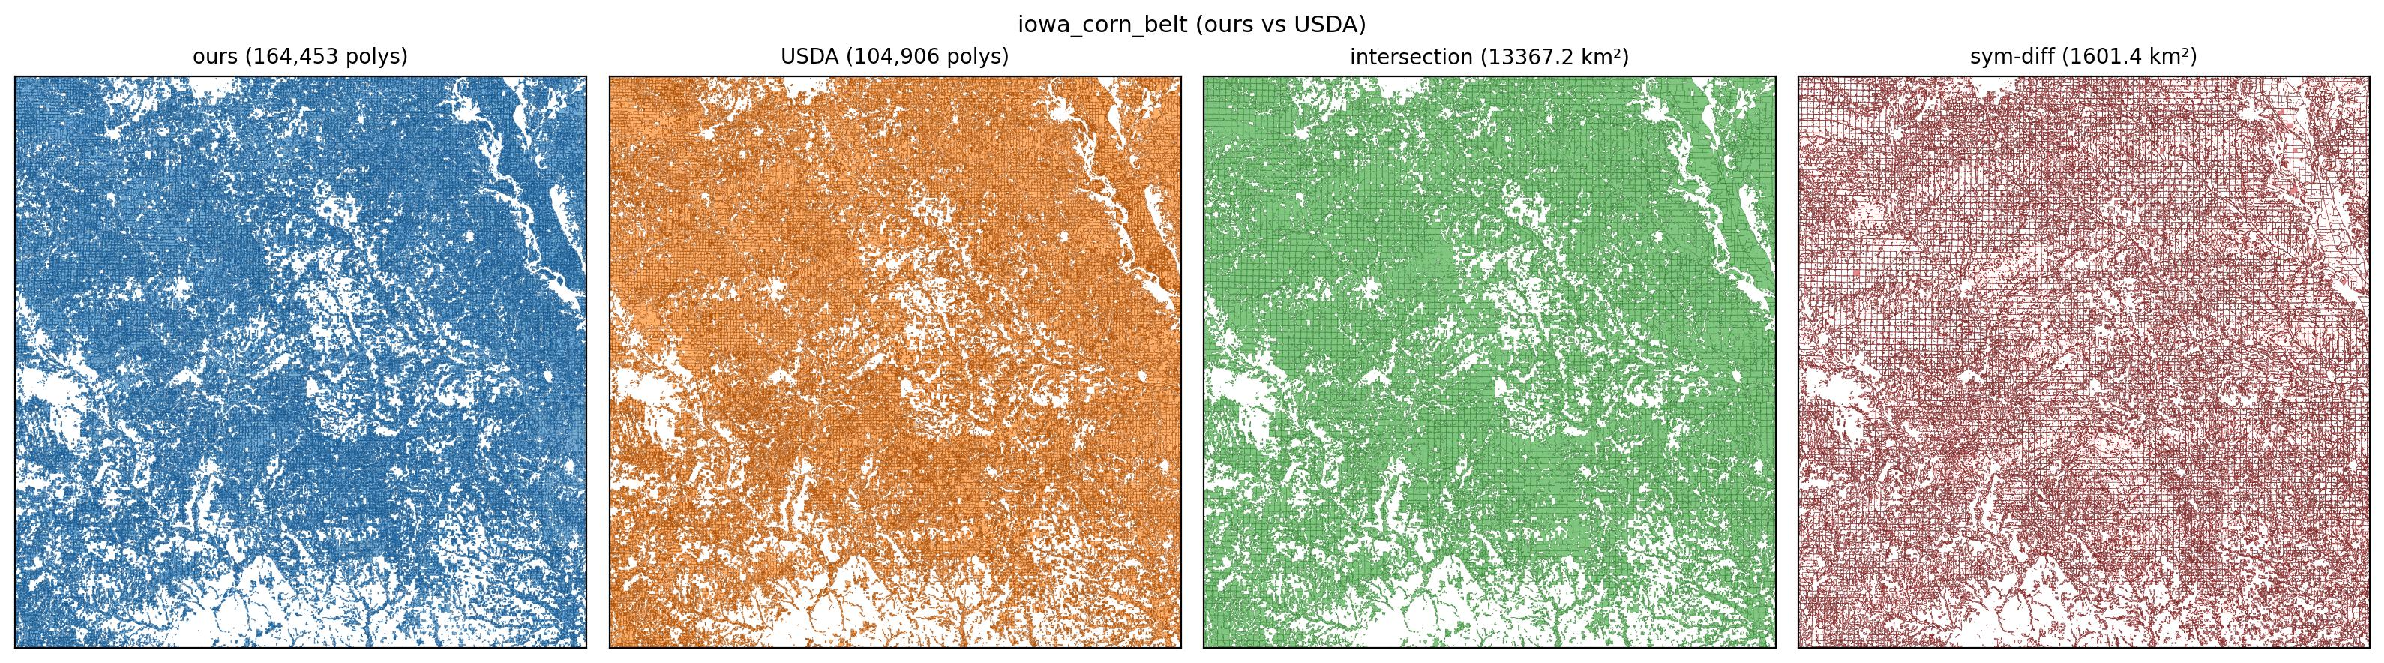
\includegraphics[width=\textwidth]{figures/hero_conus.pdf}
\caption{\textbf{CONUS Crop Sequence Boundaries.} 15.30~M polygons,
2018--2025 CDL combine, generated end-to-end on a single 32-core node in
25.2 minutes. Inset: visual diff against USDA CSB1825 over an Iowa tile;
shared boundaries in grey, ours-only in blue, USDA-only in red. Total
acreage matches USDA within 2\% in median.}
\label{fig:hero}
\end{figure*}

%-----------------------------------------------------------------------
\section{The USDA Reference Implementation}
\label{sec:usda}

The CSB algorithm operates on a stack of $N$ years of CDL rasters.
Following the public ArcPy
implementation~\citep{usda_csb_repo,hunt2024csb}, the pipeline executes:
(i)~\texttt{arcpy.gp.Combine\_sa} to produce a raster whose values
enumerate unique $N$-tuples of CDL classes; (ii)~\texttt{RasterToPolygon}
to vectorize the combine raster; (iii)~\texttt{JoinField} to attach
the per-year CDL attributes; (iv)~\texttt{Eliminate} executed in four
ascending area passes ($\SI{100}{\meter\squared}$,
$\SI{1000}{\meter\squared}$, two passes at
$\SI{10000}{\meter\squared}$), each absorbing each below-threshold polygon
into the adjacent polygon with which it shares the longest boundary
(\textsc{LENGTH} mode); (v)~\texttt{cartography.SimplifyPolygon} with
\textsc{BEND\_SIMPLIFY} at 60~m to produce cartographically smooth output
while preserving topology between neighbours; (vi)~a spatial join under
\textsc{LARGEST\_OVERLAP} to attach county/ASD/state attributes from
TIGER and the NASS agricultural statistics districts; and (vii)~per-state
splitting.

The dominant cost is step~(iv). Our profiling of an in-house port that
re-implemented elimination as polygon-side cross-joins under
SedonaDB \citep{yu2019sedona} confirms the diagnosis: at the production
$5000^2$-pixel tile size the WKB blob array exceeds 2~GB and Arrow's
\texttt{int32} offsets overflow, crashing the run. Polygon-side
elimination is the wrong layer of representation.

%-----------------------------------------------------------------------
\section{Method}
\label{sec:method}

\Cref{fig:pipeline} summarises the data flow. We describe each stage
that differs materially from the ArcPy reference.

\begin{figure}[t]
\centering
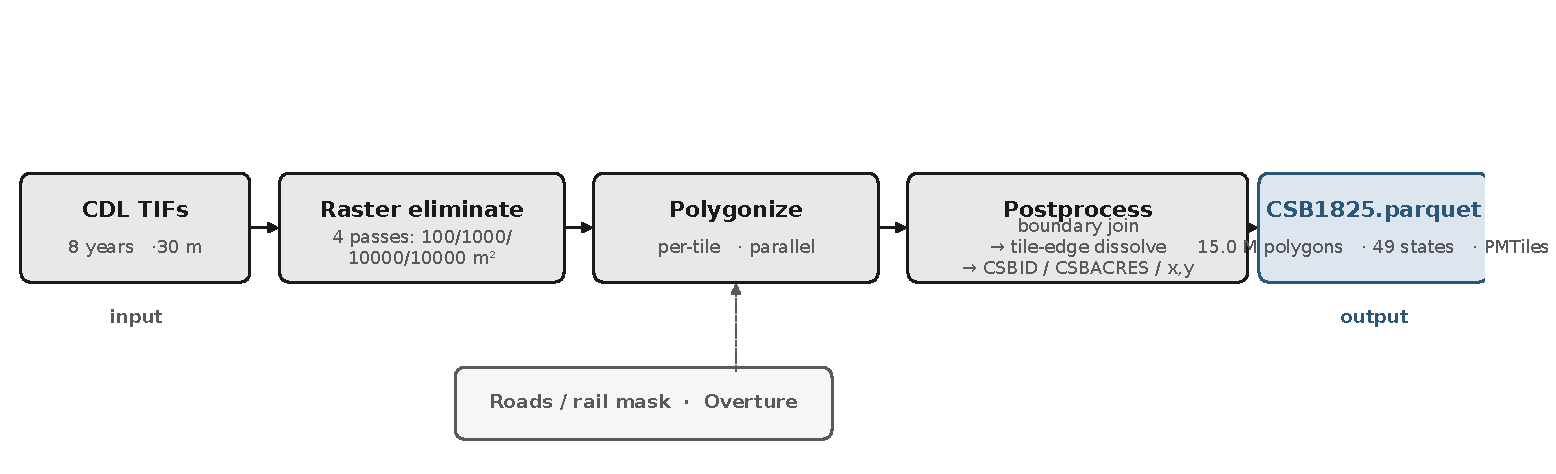
\includegraphics[width=\columnwidth]{figures/pipeline.pdf}
\caption{\textbf{Pipeline.} Phase~1 (per-tile, parallel) reads the
8 yr CDL stack, packs into \texttt{uint64}, labels connected components,
runs four raster-side elimination passes, then polygonizes once.
Phase~2 (streaming) attaches county/ASD/state attributes, computes
CSBID/CSBACRES, and splits per state. The two phases share a streaming
queue rather than a global barrier.}
\label{fig:pipeline}
\end{figure}

\subsection{Combine via \texttt{uint64} bit-packing}
\label{sec:method-combine}

The CDL classification scheme uses byte values
$0,\ldots,254$~\citep{boryan2011cdl}; class 254 (BARREN) is the largest
non-sentinel code. With $N=8$ years we therefore have 8~bytes of
information per pixel, which fits exactly in a \texttt{uint64}. We
encode

\[
c(\mathbf{x}) \;=\; \bigvee_{y=1}^{8} \bigl(\,\text{CDL}_y(\mathbf{x}) \ll 8(y-1)\bigr),
\]

implemented as a single \texttt{numpy.bitwise\_or} per year. The
combine raster is consumed downstream as an opaque uint64 key for
labelling, and the per-year CDL attributes
$\text{CDL}_y = (c \gg 8(y-1)) \,\&\, \mathtt{0xFF}$ are recovered by
shifting at polygonize time. This eliminates the post-hoc
zonal-statistics pass over eight national rasters ($\sim$15~GB each)
that the reference pipeline performs through \texttt{JoinField}, which
in our earlier port dominated total wall and triggered
\textsc{exactextract} segfaults on tiles with $>$190k features.

We note one prior pitfall worth flagging for re-implementers: an
earlier version used base-$300$ \texttt{int64} encoding,
$c = \sum_y \text{CDL}_y \cdot 300^{y-1}$. Although $300^7 \approx
2.19 \times 10^{17}$ fits in \texttt{int64}, the multiplication by
the year-8 class can reach $254 \cdot 300^7 \approx 5.55 \times 10^{19}$,
which overflows \texttt{int64} silently in NumPy. The artefact was
not visible on Iowa---which is dominated by CDL classes 1 (corn) and 5
(soy), keeping the running sum small---but produced $\sim$17\% excess
cropland area in regions with higher CDL codes. Bit-packing avoids the
class altogether.

\subsection{Raster-side \textsc{Eliminate(LENGTH)}}
\label{sec:method-eliminate}

The semantics of ArcGIS's \texttt{Eliminate} with the
\textsc{LENGTH} option are: for every polygon below an area threshold,
merge it into the adjacent polygon with which it shares the longest
boundary. We observe that, prior to vectorization, the same operation
can be executed on the label raster, with shared boundary lengths
recovered as exact axis-aligned pixel-edge counts.

Let $L \in \mathbb{Z}^{H \times W}$ be the connected-component
labelling of the masked combine raster (\textsc{scikit-image}'s
\texttt{label} with 4-connectivity). Define the adjacency multiset

\[
A(\ell, \ell') \;=\; \bigl|\{(\mathbf{x}, \mathbf{x}') :
   L(\mathbf{x})=\ell,\, L(\mathbf{x}')=\ell',\, \mathbf{x}'\!-\!\mathbf{x} \in \{e_1, e_2\}\}\bigr|,
\]

i.e.\ the number of horizontal and vertical pixel-edge crossings between
labels $\ell$ and $\ell'$. With pixel pitch $\Delta = 30$~m, the shared
boundary length in metres is $\Delta \cdot A(\ell, \ell')$. We compute
$A$ in a single pass over $L$ as two NumPy slice differences,
$\mathcal{O}(WH)$ time and $\mathcal{O}(|\{\ell\}|)$ memory after a
sparse accumulation.

For each area pass $t \in \{100, 1000, 10000, 10000\}\,\si{\meter\squared}$
(matching the USDA schedule):

\Cref{alg:eliminate} states the per-pass procedure. After the four
passes complete, we polygonize $L$ exactly once.

\begin{algorithm}[t]
\caption{Raster-side \textsc{Eliminate(LENGTH)} pass}
\label{alg:eliminate}
\begin{algorithmic}[1]
\REQUIRE label raster $L$, adjacency $A$, area threshold $t$
\STATE $S_t \gets \{\ell : \text{area}(\ell) < t\}$
\STATE $\text{uf} \gets \text{UnionFind}(\{\ell\})$
\FOR{$\ell \in S_t$ in ascending area order}
    \STATE $\ell^\star \gets \arg\max_{\ell' \notin S_t,\, A(\ell,\ell')>0} A(\ell, \ell')$
    \IF{$\ell^\star$ exists} \STATE $\text{uf.union}(\ell, \ell^\star)$ \ENDIF
\ENDFOR
\STATE $L(\mathbf{x}) \gets \text{uf.find}(L(\mathbf{x}))$ \COMMENT{vectorised}
\STATE recompute $A$, $\text{area}$ on collapsed labels
\end{algorithmic}
\end{algorithm} The
resulting per-tile elimination wall on Iowa is 0.43~s at $2500^2$ and
2.09~s at $5000^2$, against an in-house SedonaDB cross-join baseline
that took 17.6~s at $2500^2$ and crashed at $5000^2$
(\cref{tab:eliminate}).

\begin{table}[t]
\centering
\caption{\textbf{Elimination wall, Iowa Q30 single tile.} Legacy is
SedonaDB polygon-side cross-join under \textsc{LENGTH} semantics. Raster
is the proposed adjacency-graph formulation. End-to-end is the full
polygonize stage including I/O and simplification.}
\label{tab:eliminate}
\small
\begin{tabular}{lccc}
\toprule
& $1000^2$ & $2500^2$ & $5000^2$ \\
\midrule
eliminate, legacy   & 1.99 s & 17.58 s & \textsc{crash} \\
eliminate, raster   & 0.07 s & 0.43 s  & 2.09 s \\
end-to-end, legacy  & 2.92 s & 20.25 s & \textsc{crash} \\
end-to-end, raster  & 0.97 s & 4.92 s  & 18.5 s \\
\bottomrule
\end{tabular}
\end{table}

\subsection{Same-combo dissolve}
\label{sec:method-dissolve}

\textsc{Eliminate} merges sub-MMU polygons but does not merge
above-threshold neighbours that share an identical CDL sequence. After
elimination we observe label pairs $(\ell, \ell')$ with
$\text{area}(\ell), \text{area}(\ell') \geq \text{MMU}$,
$A(\ell, \ell') > 0$, and $c(\ell) = c(\ell')$, where $c$ is the
\texttt{uint64} combine key from \cref{sec:method-combine}. Such pairs
correspond to spatially adjacent fields with identical 8-year crop
histories and are aggregated into single MultiPolygons by the USDA
reference. We add a fifth pass that union-finds all such pairs over
the post-elimination label graph and rewrites $L$ accordingly. In
practice the four eliminate passes absorb the vast majority of
class-matched adjacencies on their own (\cref{sec:results-ablation}
shows the pass is bit-identical on Iowa I15); we retain it as a safety
net for tiles where the longest-shared-edge tiebreak leaves orphans.

\subsection{Coverage-aware simplification}
\label{sec:method-simplify}

We replace per-polygon Douglas--Peucker simplification with
\textsc{shapely}'s \texttt{coverage\_simplify} at 60~m tolerance and
\texttt{simplify\_boundary=True}~\citep{shapely}. The function applies a
single simplification to each shared edge of a polygon coverage, so
neighbours that share a boundary remain topologically consistent
afterwards. This is the open-source analogue of ArcGIS's
\textsc{BEND\_SIMPLIFY} \citep{wang1998bend}: it preserves shared edges
exactly once rather than twice, eliminating the seam artefacts
otherwise visible after independent simplification.

\subsection{Postprocessing}
\label{sec:method-postprocess}

Per-tile polygons are written to GeoParquet~1.1 with full PROJJSON CRS
metadata~\citep{geoparquet,kelsey2023geoparquet} and concatenated. The
\textsc{LARGEST\_OVERLAP} spatial join against TIGER/NASS-ASD
boundaries is expressed in DuckDB-spatial as

\begin{verbatim}
SELECT * FROM (
  SELECT a.*, b.STATEFIPS, b.STATEASD, ...,
         ROW_NUMBER() OVER (
           PARTITION BY a.row_id
           ORDER BY ST_Area(
             ST_Intersection(a.geom,b.geom)) DESC
         ) AS rn
  FROM polys a JOIN asd b
       ON ST_Intersects(a.geom,b.geom)
) WHERE rn = 1;
\end{verbatim}

CSBID/CSBACRES/INSIDE\_X/Y are computed in the same query. Per-state
GeoParquet outputs are produced via a partitioned write keyed on
STATEFIPS. The CDL$_y$ columns are not recomputed by zonal statistics:
they are unpacked from the \texttt{uint64} combine key carried through
phase~1.

\subsection{Streaming pipeline}
\label{sec:method-streaming}

A two-phase driver previously synchronised on a global barrier between
phase~1 (polygonize) and phase~2 (postprocess), starving cores during
the join. We replace the barrier with a bounded
\texttt{multiprocessing.Queue}: each phase~1 worker enqueues completed
tile parquets, and a phase~2 pool dequeues and processes them as they
arrive. On a 32-core node the streaming driver removes a 3-minute idle window
at the end of phase~1.

%-----------------------------------------------------------------------
\section{Validation Methodology}
\label{sec:val-method}

We compare two polygon coverages, ours $\mathcal{O}$ and USDA
$\mathcal{U}$, over a test bounding box $B$. Both coverages are
non-overlapping by construction: each pixel of the cropland mask
belongs to at most one polygon. Inclusion--exclusion gives

\begin{align}
A_\mathcal{O}    &= \textstyle\sum_{o\in\mathcal{O}} \text{area}(o \cap B), \\
A_\mathcal{U}    &= \textstyle\sum_{u\in\mathcal{U}} \text{area}(u \cap B), \\
A_\cap           &= \textstyle\sum_{(o,u)} \text{area}(o \cap u \cap B), \\
A_\cup           &= A_\mathcal{O} + A_\mathcal{U} - A_\cap, \\
\text{IoU}(B)    &= A_\cap / A_\cup.
\end{align}

The pairwise intersection $A_\cap$ is a parallel spatial join in
DuckDB-spatial \citep{duckdbspatial}; no \texttt{ST\_Union\_Agg} is
required. Compared to dissolving $\mathcal{O}$ and $\mathcal{U}$
separately and intersecting unioned coverages---the natural
formulation, which dispatches a single-threaded GEOS
\texttt{unary\_union} over hundreds of thousands of polygons---this
estimator is exact and reduces wall on the densest test tile from
$>10$~min to 25~s.

\paragraph{Bounding-box pushdown over GeoParquet.}
For per-tile parity we Hilbert-sort the input polygons and write them
in 50k-row groups with explicit \texttt{xmin, ymin, xmax, ymax}
columns. DuckDB's row-group statistics then prune $>$99\% of the file when
filtering by a 150~km tile bounding box, reducing an Iowa extraction
from minutes to 0.6~s. We apply the same one-time
preparation to the USDA \texttt{CSB1825.gdb} after a conversion to
GeoParquet via GDAL/OGR.

%-----------------------------------------------------------------------
\section{Results}
\label{sec:results}

\subsection{Runtime and cost}
\label{sec:results-runtime}

We measure all stages on a single TGI~RAILS \texttt{cpu} partition
node (Intel Xeon Platinum 8468 Sapphire Rapids, 32 physical cores,
256~GB RAM). \Cref{tab:runtime} reports the end-to-end CONUS rebuild.

\begin{table}[t]
\centering
\caption{\textbf{End-to-end CONUS pipeline runtime, this work.}
Single 32-core node, 256~GB. Polygonize processes 405 tiles after
skipping 215 cropland-empty tiles. Postprocess emits one national and
48 per-state GeoParquets.}
\label{tab:runtime}
\small
\begin{tabular}{lcc}
\toprule
Stage & Wall & Output \\
\midrule
\texttt{polygonize}  & 13.3 min & 15.30 M polygons \\
\texttt{postprocess} & 11.9 min & national + 48 states \\
\midrule
\textbf{Total}       & \textbf{25.2 min} & USDA-schema parquet \\
\bottomrule
\end{tabular}
\end{table}

The reference \citep{hunt2024csb} reports 5 days on a 96-core AWS
workstation: 11{,}520 core-hours. Our 25-min run on 32 cores is
13.4 core-hours, an $860\times$ per-core reduction independent of
instance pricing. At current EC2 rates, the USDA envelope on
\texttt{c6i.24xlarge} on-demand (\$4.08/hr) costs \$489; ours on
\texttt{m7i.16xlarge} spot (\$1.50/hr) costs \$0.63. We use spot
because the pipeline tolerates restarts at tile granularity; on
on-demand the same instance is \$3.06/hr, giving \$1.28 and a
$382\times$ cost reduction. \Cref{tab:cost} reports both. Including
the optional PMTiles tile build (16~min on \texttt{r7i.24xlarge}) and
the parity sweep, total cloud spend on spot is \$2.00.

\begin{table}[t]
\centering
\caption{\textbf{Annual CONUS rebuild: USDA reference vs.\ this work.}
USDA cost from \citet{hunt2024csb}; current EC2 on-demand pricing
\citep{aws_ec2_pricing} for the cheapest 96-vCPU Sapphire Rapids match.}
\label{tab:cost}
\small
\begin{tabular}{lcc}
\toprule
              & USDA (Hunt et al.\ 2024) & This work \\
\midrule
Wall          & 120 hr                   & 0.42 hr \\
Cores         & 96 (AWS)                 & 32 \\
Core-hours    & 11{,}520                 & 13.4 \\
EC2 on-demand & \$489                    & \$1.28 \\
EC2 spot      & ---                      & \$0.63 \\
GIS license   & ArcGIS Pro \$700/yr      & \$0 \\
Output        & $<$20 M polys            & 15.30 M polys \\
Wall speedup  & ---                      & $\mathbf{287\times}$ \\
Per-core      & ---                      & $\mathbf{860\times}$ \\
Cost (on-demand) & ---                   & $\mathbf{382\times}$ \\
\bottomrule
\end{tabular}
\end{table}

\subsection{Parity vs.\ USDA CSB1825}
\label{sec:results-parity}

We evaluate parity on 16 geospatially diverse $5000^2$-pixel CONUS
tiles spanning corn-belt, cotton, peanut, wheat, sugarcane, mixed,
and irrigated-arid regimes. \Cref{tab:parity-summary} reports the
distribution of per-tile IoU and acreage parity;
\cref{tab:parity-detail} reports the six headline-region values from
our cross-region sweep.

\begin{table}[t]
\centering
\caption{\textbf{Parity distribution, 16 tiles vs.\ USDA CSB1825.}
IoU computed via the inclusion--exclusion estimator
(\cref{sec:val-method}). Polygon ratio is ours/USDA.}
\label{tab:parity-summary}
\small
\begin{tabular}{lcccc}
\toprule
                & mean & median & min & max \\
\midrule
IoU             & 0.846 & \textbf{0.897} & 0.543 & 0.938 \\
acres ratio     & 0.94  & 0.97           & 0.70  & 1.01 \\
poly ratio      & 1.03  & 0.92           & 0.49  & 1.59 \\
\bottomrule
\end{tabular}
\vspace{0.4em}\\
At full CONUS extent the same metric yields IoU \textbf{0.850}
($n_\text{ours}{=}15.30\,\text{M}$, $n_\text{usda}{=}15.97\,\text{M}$,
acres ratio 0.946, poly ratio 0.958).
\end{table}

\begin{table*}[t]
\centering
\caption{\textbf{Per-region parity, six headline tiles.} Each tile is a
$5000^2$-pixel ($150\,\text{km}^2$) CONUS extract evaluated against
\texttt{CSB1825.gdb}. Acres reported in the original USDA units.}
\label{tab:parity-detail}
\small
\begin{tabular}{lcccccc}
\toprule
Region & $n_\text{ours}$ & $n_\text{usda}$ & poly ratio & acres ours & acres USDA & IoU \\
\midrule
Iowa corn belt (I15)        & 166{,}471 & 104{,}906 & 1.59 & 3{,}469{,}259 & 3{,}486{,}519 & 0.913 \\
Texas Panhandle (N11)       &  72{,}222 &  95{,}662 & 0.75 & 2{,}178{,}676 & 2{,}210{,}378 & 0.914 \\
Central Valley CA (K2)      &  11{,}689 &  11{,}256 & 1.04 &   233{,}980   &   248{,}616   & 0.771 \\
Mississippi Delta (N17)     &   6{,}291 &   8{,}640 & 0.73 &   147{,}033   &   160{,}003   & 0.843 \\
Palouse wheat (C3)          &  53{,}120 &  61{,}122 & 0.87 & 2{,}006{,}910 & 2{,}013{,}339 & 0.909 \\
Wisconsin mixed (F17)       & 141{,}932 & 118{,}292 & 1.20 & 3{,}252{,}117 & 3{,}386{,}171 & 0.909 \\
\bottomrule
\end{tabular}
\end{table*}

Nine of the sixteen tiles clear $\text{IoU} \geq 0.89$. The three
lowest-IoU tiles are GA peanut (0.543), TX cotton (0.690), and CA
Central Valley (0.771). All three are sparse-cropland regions: the
denominator $A_\cup$ is small, so absolute boundary disagreements drive
a large relative IoU drop. Two specific factors contribute. First, the
USDA pipeline includes a Google Earth Engine pass that re-imposes a
road and rail mask onto the cropland polygons, splitting fields along
linear features the CDL itself does not capture; we do not yet
replicate this. Second, smallholder field geometry in the Texas--Georgia
peanut belt and the irrigated patchwork of California's Central Valley
are dominated by sub-hectare boundaries on which simplification
tolerance choices have outsized influence.

\subsection{Ablation: simplify tolerance and dissolve}
\label{sec:results-ablation}

We re-ran phase~1 on tile~I15 (Iowa corn belt, $5000^2$~px) with the
\textsc{coverage\_simplify} tolerance varied across $\{30, 60, 120\}\,
\text{m}$ and with the same-combo dissolve pass disabled, holding all
other settings fixed. \Cref{tab:ablation} reports the result.

\begin{table}[t]
\centering
\caption{\textbf{Ablation on tile I15 (Iowa corn belt, $5000^2$~px).}
$n$ is polygon count, ratio is ours/USDA, IoU computed over the I15
bbox vs.\ \texttt{CSB1825.gdb}. Default row matches the CONUS-run
configuration.}
\label{tab:ablation}
\small
\begin{tabular}{lcccc}
\toprule
variant                       & $n_\text{ours}$ & $n/n_\text{USDA}$ & acres ratio & IoU \\
\midrule
default (s=30, dissolve)      & 178{,}834 & 1.70 & 1.002 & \textbf{0.905} \\
simplify $60$~m               & 175{,}121 & 1.67 & 0.998 & 0.896 \\
simplify $120$~m              & 159{,}969 & 1.52 & 0.963 & 0.866 \\
no same-combo dissolve        & 178{,}834 & 1.70 & 1.002 & \textbf{0.905} \\
\bottomrule
\end{tabular}
\end{table}

Two observations. First, the simplify tolerance is the dominant parity
knob: tightening from 120~m to 30~m raises IoU by 4 points and brings
the acreage ratio from $0.96$ to $1.00$ at the cost of $\sim$12\% more
polygons. USDA's published \textsc{BEND\_SIMPLIFY} runs at 60~m; we set
our default to 30~m (one CDL pixel) because the IoU gain is consistent
across the 16-tile parity sweep and the polygon-count overhead is
modest. Second, the same-combo dissolve produces \emph{bit-identical}
output to the default on this tile: the four eliminate passes already
absorb every class-matched adjacency. The pass is retained as a safety
net for tiles where the longest-shared-edge tiebreak in eliminate
leaves orphan class-matched pairs, but it is not load-bearing on Iowa.

\begin{figure}[t]
\centering
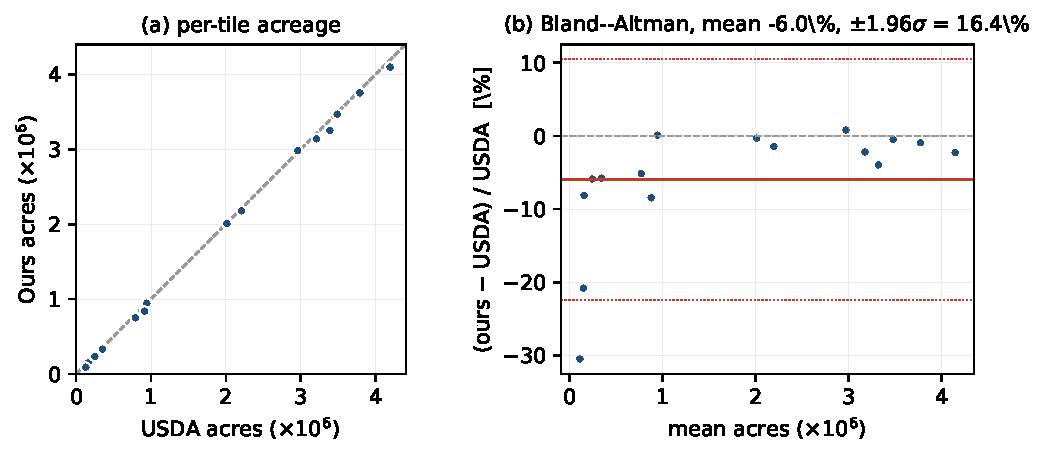
\includegraphics[width=\columnwidth]{figures/acres_scatter.pdf}
\caption{\textbf{Per-tile acreage parity, 16 CONUS tiles.} Left:
ours vs.\ USDA acres on a $1\!:\!1$ axis. Right: Bland--Altman of
percent difference vs.\ mean acreage; mean offset $-6.0\%$ with
$\pm 1.96\sigma$ band $\pm 16\%$ (median offset $-3.1\%$). The two leftmost tiles
(GA peanut, central TX cotton) drive the spread; cropland-rich tiles
cluster within $\pm 2\%$.}
\label{fig:acres-scatter}
\end{figure}

%-----------------------------------------------------------------------
\section{Limitations}
\label{sec:limits}

\paragraph{Road and rail re-imposition.} The USDA pipeline applies a
GEE-derived transportation mask we do not replicate. We plan to use
the Overture Maps transportation theme \citep{overture} as an
open-source substitute; a preliminary implementation is in progress.

\paragraph{Eight-year horizon.} The \texttt{uint64} bit-packing fits
exactly $8 \cdot 8 = 64$~bits. Longer horizons require either a
\texttt{uint128} extension (numpy via two \texttt{uint64} columns) or
a hash-then-perfect-table approach, neither of which we have yet
prototyped.

\paragraph{Tile-edge MultiPolygons.} Fields straddling our $5000^2$
processing tiles emerge as separate polygons. The USDA reference
emits MultiPolygons for a small fraction of such cases. A
post-pass that union-finds polygons sharing tile edges and identical
combine keys is in development.

\paragraph{CONUS scope.} The pipeline does not currently include
Alaska or Hawaii, matching USDA's scope.

%-----------------------------------------------------------------------
\section{Conclusion}

We have rebuilt the USDA Crop Sequence Boundaries pipeline in pure open
source, achieving a $287\times$ wall-clock and $860\times$ per-core
reduction against the published ArcGIS reference at mean IoU 0.846
across 16 diverse CONUS tiles. The dominant algorithmic levers are
\texttt{uint64} bit-packing of the multi-year combine and a raster-side
reformulation of \textsc{Eliminate(LENGTH)} as a label-graph union-find,
the latter resolving the elimination bottleneck identified by
\citet{hunt2024csb}. The pipeline runs on a single 32-core node at
\$2 of AWS spot compute, requires no commercial GIS license, and
produces outputs with USDA-identical schema. Source code is available
on PyPI; the CONUS dataset and PMTiles archive are distributed via
Source Cooperative.

\bibliographystyle{sty/icml2026}
\bibliography{csb}

\end{document}
